\chapter{Background}

\section{Kubernetes}
\textbf{Kubernetes}~\cite{kubernetes} (k8s) is an open-source system for
automating deployment, scaling, and management of containerized applications.

\section{Technologies}
Kubernetes is written in Go~\cite{golang} (also called golang)~\cite{golang-info}
--- an open source compiled, statically typed imperative language created by
Google engineers Rob Pike, Robert Griesemer and Ken Thompson in 2012. It was
meant for concurrent computing and distributed systems programming. Golang is
broadly used in cloud-based projects, such as Google Cloud, AWS,
Microsoft Azure, Digital Ocean, or Heroku.


\section{Structure}
\subsection{Cluster}
A cluster is a single logical unit consisting of a group of computers working
together. A  single machine with its own operating system linked to other
components within a cluster is called a \emph{node}. Kubernetes clusters provide
us with an efficient way of deploying applications with automated distribution
across a cluster using containerization. Nodes within a cluster have different
roles. The primary distinction is that of \emph{master} and \emph{worker} nodes.
There is one master node, responsible for orchestrating the cluster and keeping
track of state necessary to accomplish this goal. Business logic is performed
by the worker nodes, created dynamically to fulfill the requests from users.

\begin{figure}[!ht]
    \centering
    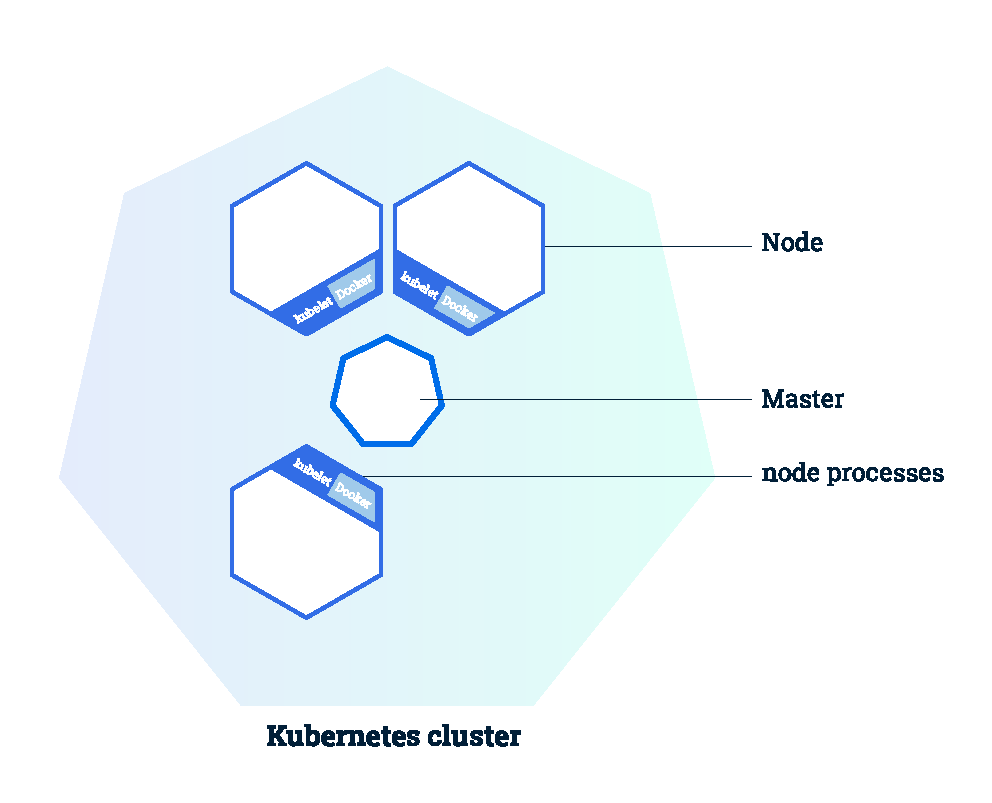
\includegraphics[width=0.4\textwidth, angle=0]{img/kubernetes_cluster.pdf}
\end{figure}

\subsection{Master}
The master node~\cite{master-node} is responsible for processing events in the
cluster and making global decision, such as scheduling and scaling. The master
usually runs on a computer separate from the ones dedicated to hosting worker
jobs. It consists of several components that allow for communication between
other nodes and cluster users. It also manages resources for the worker nodes.

\subsection{Kube-apiserver}
One of the most important features of the master node is a server running on it,
exposing a RESTful API. The API may be queried by users and applications to get
information about the cluster’s current state, and requests can be made to
request the addition, deletion, or modification of various API objects. As
requests are made, a \emph{desired} state is defined. It is the job of other
processes running on the master node to make the \emph{actual} state match this
desired state.

\subsection{Etcd}
Etcd is a daemon providing a dynamic key-value configuration registry. The
master node uses etcd to store information about the cluster’s state. Requests
to the kubernetes apiserver result in queries and modifications of the data
stored in etcd.

\subsection{Kube-controller-manager}
Another vital part of the master node is a group of controllers that manage
cluster work. These are the processes responsible for making the actual state
match the desired state, as stored in etcd.

\subsection{Pod}
A pod is an abstraction for one or more containers with shared resources like
volumes or network. Each pod within a cluster has a lifecycle. From creation,
a pod is tied to a specific node by the scheduler and runs there until
termination. In the event of a node failing, the pod will be recreated on a new,
working node. It is an “atomic” unit in the Kubernetes cluster.

Kubelet is a program running on every node. It is responsible for managing pods
and communication with the master.

\subsection{Kubectl}
Kubectl is a command-line interface used for accessing core kubernetes
functionalities and interacting with a cluster.

\section{Expanding the Kubernetes API}
Kubernetes was designed to be easily extensible and
configurable~\cite{extending-kubeapi}. There are many ways of customizing the
API and adding new functionalities, so called Custom Resources. The idea behind
Custom Resources is to allow the user to define new API objects that can be
handled in the same way as resources already understood by Kubernetes. As
a result, they provide a way of customizing a specific Kubernetes installation,
exposing new behavior that can be accessed via the same kubectl operations as
default resources.

\subsection{Aggregation Layer}
The basic way of expanding the k8s API, introduced in kubernetes 1.7, is using
the aggregation layer. Thanks to this tool, one can perform API aggregation at
runtime. The aggregation layer enables the creation of custom resources by
deploying its own API server.

\subsection{Custom Resource Definitions}
Custom Resource Definitions (CRDs) are another way of defining custom resources.
A user can create a Custom Resource Definition object in the API, specifying
a name and schema for the type of custom resource they wish to introduce.
Custom Resource Definitions are static objects in the API. Once a CRD exists,
Custom Resource objects of the defined type can be created by users. This way
of creating Custom Resources provides developers with less flexibility than
aggregation layers but requires less overhead for simple applications.
